% Defino el tipo de hoja y documento.
\documentclass[titlepage,a4paper]{article}

% Importo los paquetes, defino encabezado, pie de pagina y margenes.
\usepackage{a4wide}
\usepackage[left=1.27cm, right=1.27cm, top=2.5cm, bottom=2.5cm, headheight=1.25cm]{geometry}
\usepackage[colorlinks=true,linkcolor=black,urlcolor=blue,bookmarksopen=true]{hyperref}
\usepackage{bookmark}
\usepackage{fancyhdr}
\usepackage[spanish]{babel}
\usepackage[utf8]{inputenc}
\usepackage[T1]{fontenc}
\usepackage{graphicx}
\usepackage{float}

% Creo el encabezado y pie de página
\pagestyle{fancy} 
\fancyhf{}
\fancyhead[L]{TP1 - Federico N. Pratto}
\fancyhead[R]{Algoritmos y Programación III - FIUBA}
\renewcommand{\headrulewidth}{0.4pt}
\fancyfoot[C]{\thepage}
\renewcommand{\footrulewidth}{0.4pt}

\begin{document}
\begin{titlepage} % Carátula
	\hfill
\includegraphics[width=6cm]{logofiuba.jpg}
    \centering
    \vfill
    \Huge \textbf{Trabajo Práctico 1 — Smalltalk}
    \vskip2cm
    \Large [75.07/95.02] Algoritmos y Programación III\\
    Curso 1 \\
    Segundo cuatrimestre de 2019 
    \vfill
    \begin{tabular}{ | l | l | } % Datos del alumno
      \hline
      Alumno: &  Federico N. Pratto \\ \hline
      Número de padrón: & 96.223 \\ \hline
      Email: & fede.pratto@gmail.com \\ \hline
  	\end{tabular}
    \vfill
    \vfill
\end{titlepage}

\tableofcontents % Índice general
\newpage

\section{Introducción}\label{sec:intro}
El presente informe reúne la documentación de la solución del primer trabajo práctico de la materia Algoritmos y Programación III que consiste en desarrollar una aplicación de un sistema de chat en Pharo utilizando los conceptos del paradigma de la orientación a objetos vistos hasta ahora en el curso.

\section{Supuestos}\label{sec:supuestos}
% Deberá contener explicaciones de cada uno de los supuestos que el alumno haya tenido que adoptar a partir de situaciones que no estén contempladas en la especificación.

Supuse que el usuario que utilice el chat no instanciara, de forma directa, objetos de ninguna clase que no sea la de \textit{AlgoChat}.\\
Ademas se supuso que, el usuario no cometerá errores al utilizar el programa cuando se trate de tipos de clases. Por ejemplo, si un mensaje espera recibir un objeto de la clase \textit{ByteString}, el usuario no ingresara uno de la clase \textit{SmallInteger}.\\
Luego, supuse que al crear una \textit{Conversacion}, el constructor recibirá al menos un \textit{Usuario}.

\newpage
\section{Diagramas de clase}\label{sec:diagramasdeclase}
% Uno o varios diagramas de clases mostrando las relaciones estáticas entre las clases.  Puede agregarse todo el texto necesario para aclarar y explicar su diseño. Recuerden que la idea de todo el documento es que quede documentado y entendible cómo está implementada la solución.

\begin{figure}[H]
	\centering
	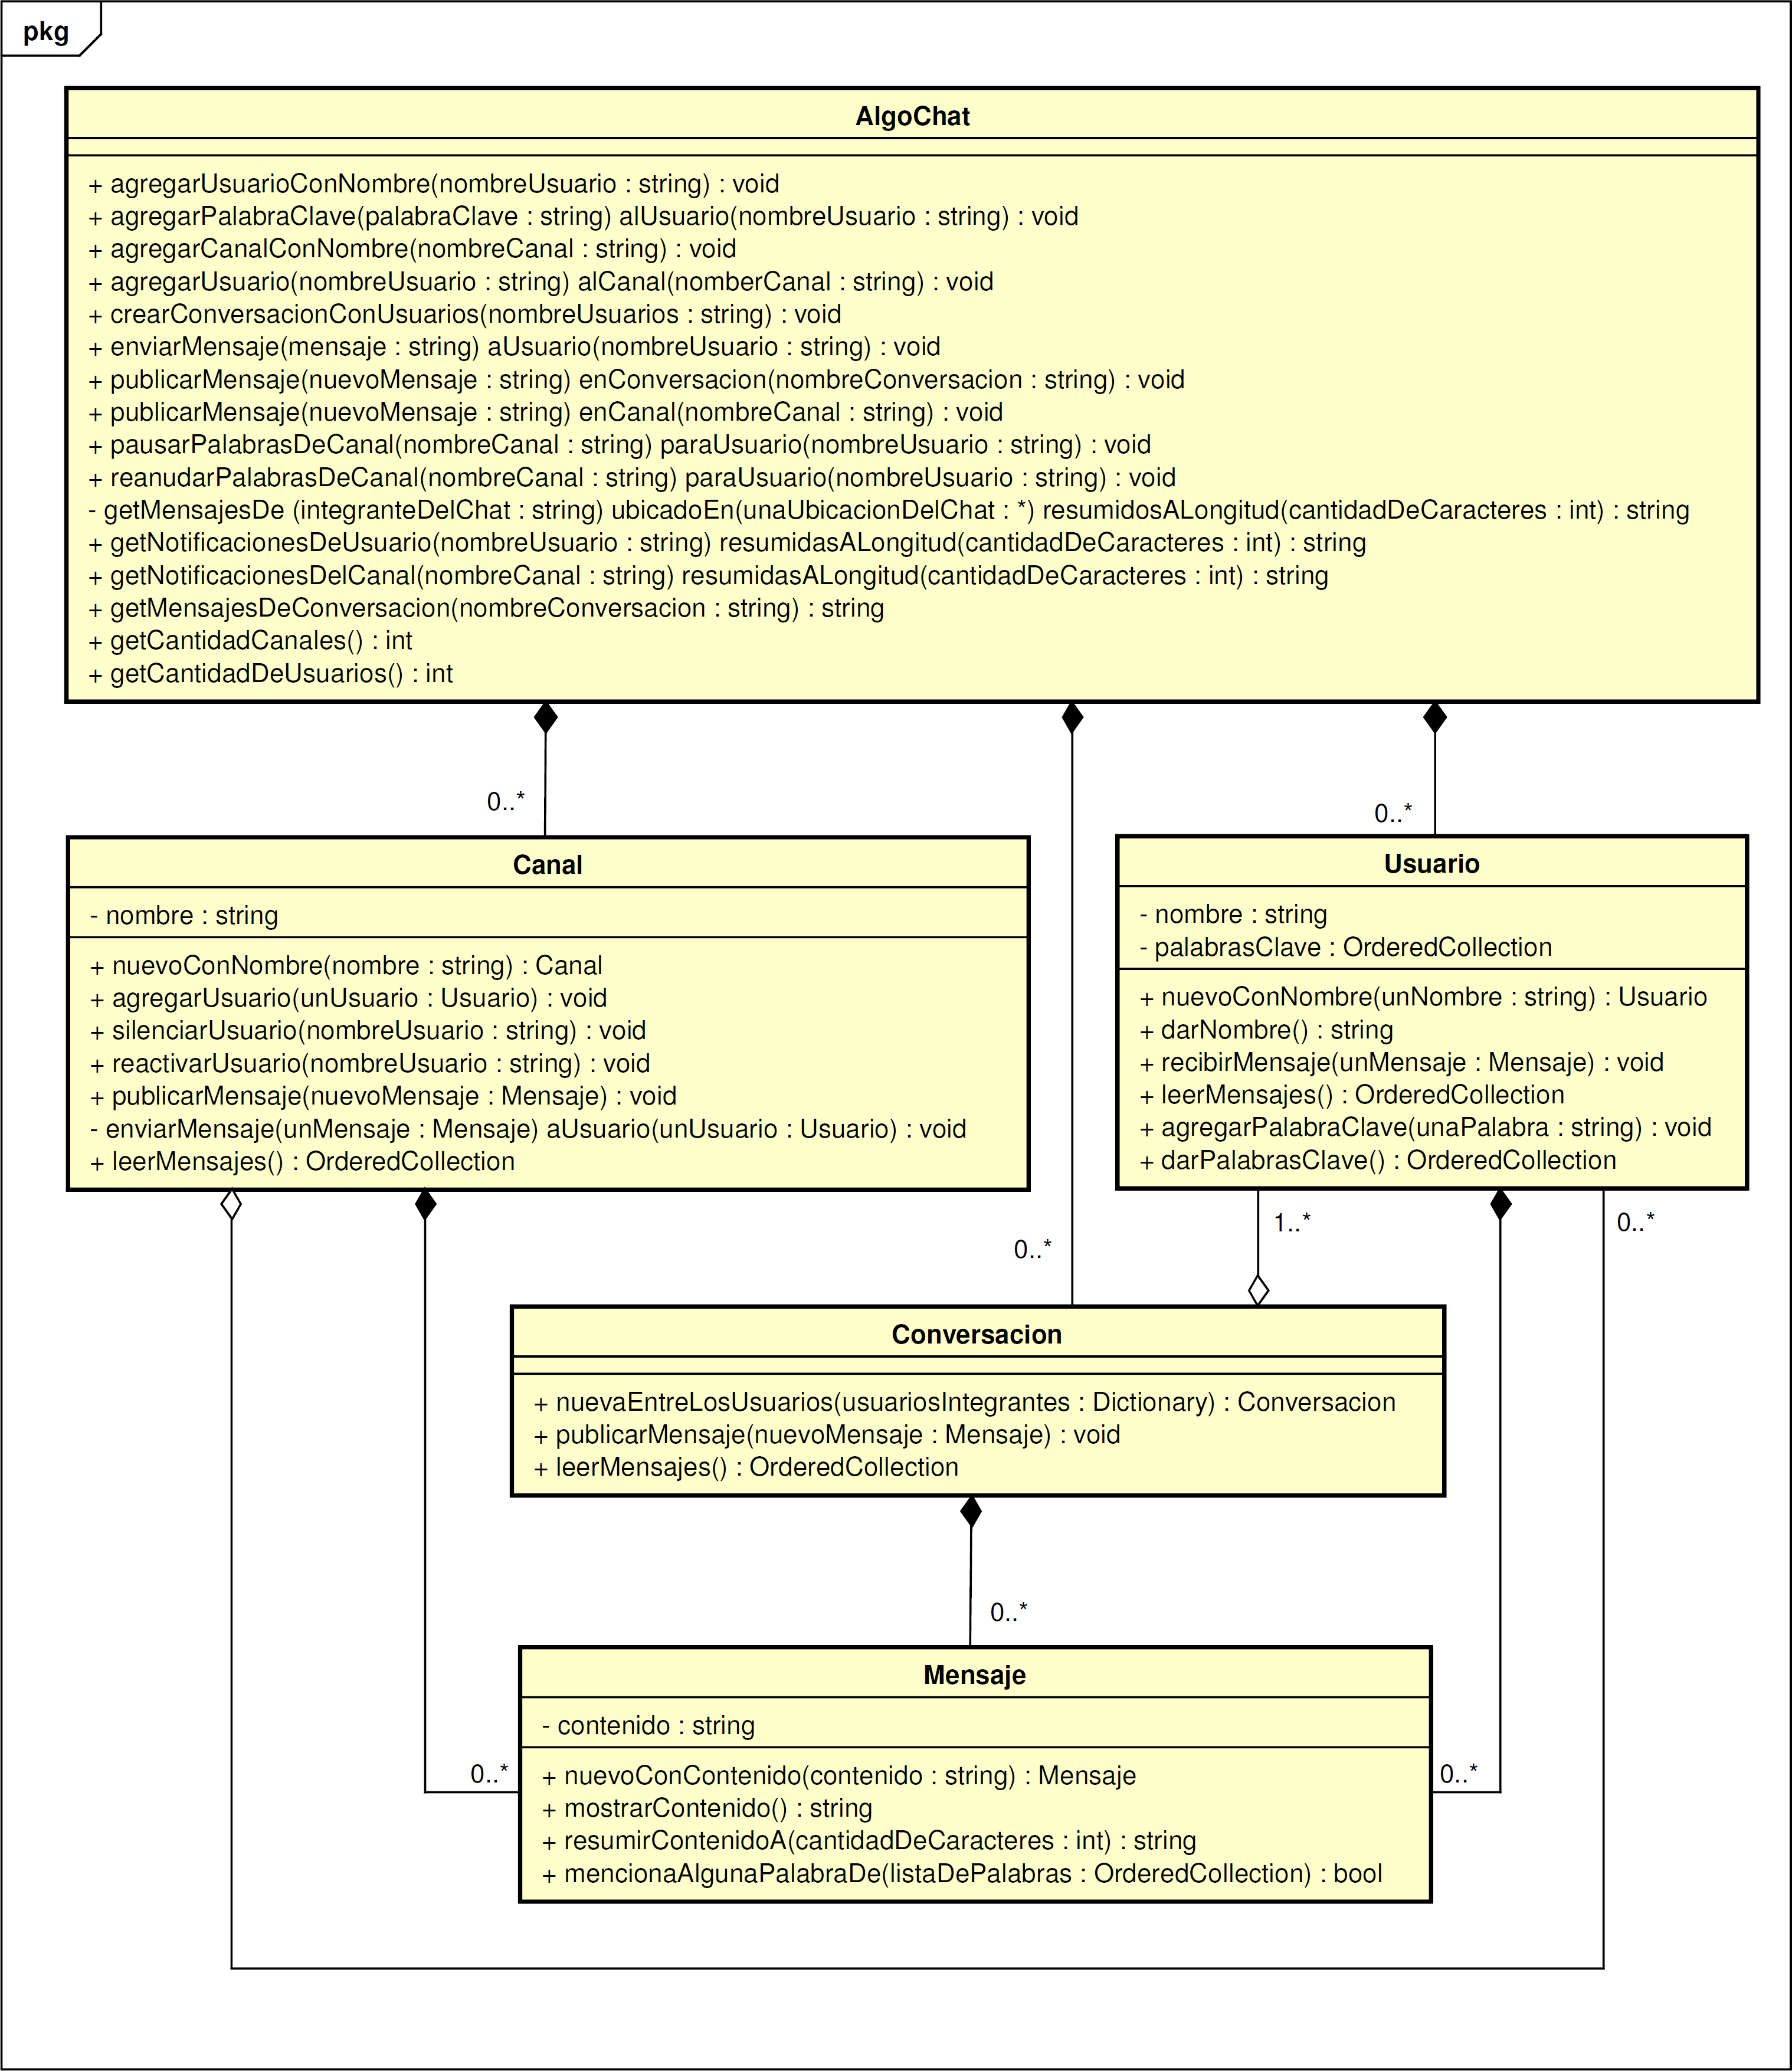
\includegraphics[width=1\textwidth]{diagrama_clase01.png}
	\caption{\label{fig:class01}Diagrama de clases general.}
\end{figure}

La resolución del trabajo consiste en cinco clases las cuales colaboran entre si de la siguiente manera:

\subsection{Usuario}\label{subsec:usuario}

Clase a partir de la cual crearemos nuevos objetos \textit{Usuario} para integrar nuestro chat, y cuyas responsabilidades serán:

\begin{itemize}
	\item Recibir un objeto \textit{Mensaje}, y almacenarlo en un listado, donde estarán todos los \textit{Mensajes} que el \textit{Usuario} haya recibido desde su creación.
	\item Indicar cual es su nombre.
	\item Devolver un listado con todos sus \textit{Mensajes}.
	\item Recibir una palabra clave, y almacenarla en un listado, para ser notificado si esta es mencionada en un \textit{Canal} al que pertenezca.
	\item Devolver un listado con todas sus palabras clave. 
\end{itemize}

Ademas de esto, el \textit{Usuario} podrá ser agregado a través del \textit{AlgoChat} tanto a \textit{Canales} como \textit{Conversaciones}, con otros de su mismo tipo.

\subsection{Canal}\label{subsec:canal}

Clase a partir de la cual se podrán crear \textit{Canales} de anuncios en el chat, estos consistirán básicamente en un lugar del chat con un nombre en particular (Por ejemplo: 'Anuncios') donde se podrán publicar \textit{Mensajes}. Y cuyas responsabilidades serán:

\begin{itemize}
	\item Aceptar a un nuevo \textit{Usuario} que podra ser agregado al \textit{Canal}.
	\item Recibir un \textit{Mensaje}, y almacenarlo en un listado, donde estarán todos los \textit{Mensajes} que se publicaron en el \textit{Canal} desde su creación.
	\item Al recibir un nuevo \textit{Mensaje}, deberá enviar el mismo a sus \textit{Usuarios}, si es que estos son mencionados (@nombreUsuario) o aparece alguna de las palabras clave, que hayan activado previamente, en el contenido del \textit{Mensaje}.
	\item Silenciar un \textit{Usuario}. Al hacer esto el \textit{Usuario} en cuestión dejara de recibir notificaciones si alguna de las palabras clave que el activo son mencionadas en un el contenido de un \textit{Mensaje}, pero continuara siendo informado si es mencionado su nombre.
	\item Reactivar a un \textit{Usuario}, esto consiste básicamente en volver a notificar al \textit{Usuario} si sus palabras claves son mencionadas en futuros \textit{Mensajes}.
	\item Devolver un listado con todos sus \textit{Mensajes}.
\end{itemize}

Una peculiaridad con respecto a como se almacenan los \textit{Usuarios} dentro de un \textit{Canal}, para hacer lo mas eficiente posible el saber quien ha sido silenciado y quien no, puede leerse en la \textbf{sección \ref{subsec:implementacionCanal}}.

\subsection{Conversacion}\label{subsec:conversacion}

Clase a partir de la cual se podrán crear \textit{Conversaciones} entre \textit{Usuarios} en el chat. Estas consistirán en un lugar donde se podrán publicar \textit{Mensajes}, los cuales serán recibidos por todos los integrantes de la \textit{Conversación}. Sus responsabilidades son las siguientes:

\begin{itemize}
	\item Recibir un \textit{Mensaje}, y almacenarlo en un listado, donde estarán todos los \textit{Mensajes} que se publicaron en la \textit{Conversación} desde su creación.
	\item Al recibir un nuevo \textit{Mensaje}, deberá reenviar el mismo a todos sus \textit{Usuarios}.
	\item Devolver un listado con todos sus \textit{Mensajes}.
\end{itemize}

\subsection{Mensaje}\label{subsec:mensaje}

Clase a partir de la cual se podrán crear \textit{Mensajes} para ser enviados a \textit{Usuarios}, \textit{Conversaciones} o \textit{Canales}. Sus responsabilidades son las siguientes:

\begin{itemize}
	\item Devolver su contenido, es decir, el texto que lo compone.
	\item Devolver su contenido resumido a una determinada cantidad de caracteres solicitada. Si la dicha cantidad es menor o igual a cero, el \textit{Mensaje} devolverá su contenido sin resumir.
	\item Indicar si una palabra que recibe aparece mencionada en su contenido.
\end{itemize}

\subsection{AlgoChat}\label{subsec:algochat}

Clase a partir de la cual sera instanciado el Chat, sus responsabilidades son:

\begin{itemize}
	\item Crear nuevos \textit{Usuarios}, \textit{Conversaciones} y \textit{Canales} en el Chat.
	\item Dotar de \textit{Usuarios} a un \textit{Canal}.
	\item Enviar mensajes a \textit{Usuarios}, \textit{Conversaciones} y \textit{Canales} en el Chat.
	\item Solicitar a un \textit{Canal} que pause o reactive las notificaciones por palabra clave de un \textit{Usuario} determinado.
	\item Devolver los mensajes de un \textit{Usuario}, \textit{Conversacion} o \textit{Canal} resumidos o no a una cierta cantidad de caracteres.
\end{itemize}

\section{Detalles de implementación}\label{sec:implementacion}
% Explicaciones sobre la implementación interna de algunas clases que consideren que puedan llegar a resultar interesantes.

\subsection{Canal: Almacenamiento de Usuarios}\label{subsec:implementacionCanal}

Al momento de almacenar los \textit{Usuarios} que se van agregando al \textit{Canal} decidí hacerlo de la siguiente manera:
\\
\begin{verbatim}
agregarUsuario: unUsuario

    | usuario |

    usuario := Array new: 2.
    usuario at: 1 put: unUsuario.
    usuario at: 2 put: 'activo'.

    usuarios at: (unUsuario darNombre) ifAbsentPut: usuario.
    
\end{verbatim}

El \textit{Canal} recibe al objeto \textit{unUsuario}, y lo almacena en el primer indice de un nuevo \textit{Array} de dos elementos. Luego, en el segundo indice de dicho \textit{Array} se almacena el estado del \textit{Usuario} dentro del \textit{Canal} (activo/silenciado).

Dicho estado sera por definición activo cuando se agrega un nuevo \textit{Usuario}, e ira mutando a lo largo de la ejecución del programa en función de si el \textit{Usuario} es silenciado o reactivado, para ese \textit{Canal} en particular.

Finalmente, se almacena este \textit{Array} en el \textit{Dictionary}, al que referencia el atributo \textit{usuarios} del \textit{Canal}, utilizando como clave el nombre del \textit{Usuario}. Si ya habia una clave con dicho valor en \textit{usuarios} (Es decir, el \textit{Usuario} ya pertenece al \textit{Canal}) no se almacena el \textit{Array}. 

\subsection{Conversación}\label{subsec:implementacionConversacion}

La \textit{Conversacion} estará compuesta en su estructura por:

\begin{itemize}
	\item Una \textit{OrderedCollection} donde se almacenaran los objetos \textit{Mensaje} en el orden que sean recibidos.
	\item Un \textit{Dictionary} donde se almacenaran los \textit{Usuarios} que integren la \textit{Conversacion} segun:
	\subitem clave: \textit{nombreDelUsuario} \quad-->\quad valor: \textit{Usuario}.
\end{itemize}

\subsection{Usuario}\label{subsec:implementacionUsuario}

Un usuario estará compuesto en su estructura por:

\begin{itemize}
	\item Un \textit{String} representando el nombre.
	\item Una \textit{OrderedCollection} donde se almacenaran los objetos \textit{Mensaje} en el orden que sean recibidos.
	\item Una \textit{OrderedCollection} donde se almacenaran las palabras clave que se le vayan agregando.
\end{itemize}

\section{Diagramas de secuencia}\label{sec:diagramasdesecuencia}
% Mostrar las secuencias interesantes que hayan implementado. Pueden agregar texto para explicar si algo no queda claro.

\begin{figure}[H]
\centering
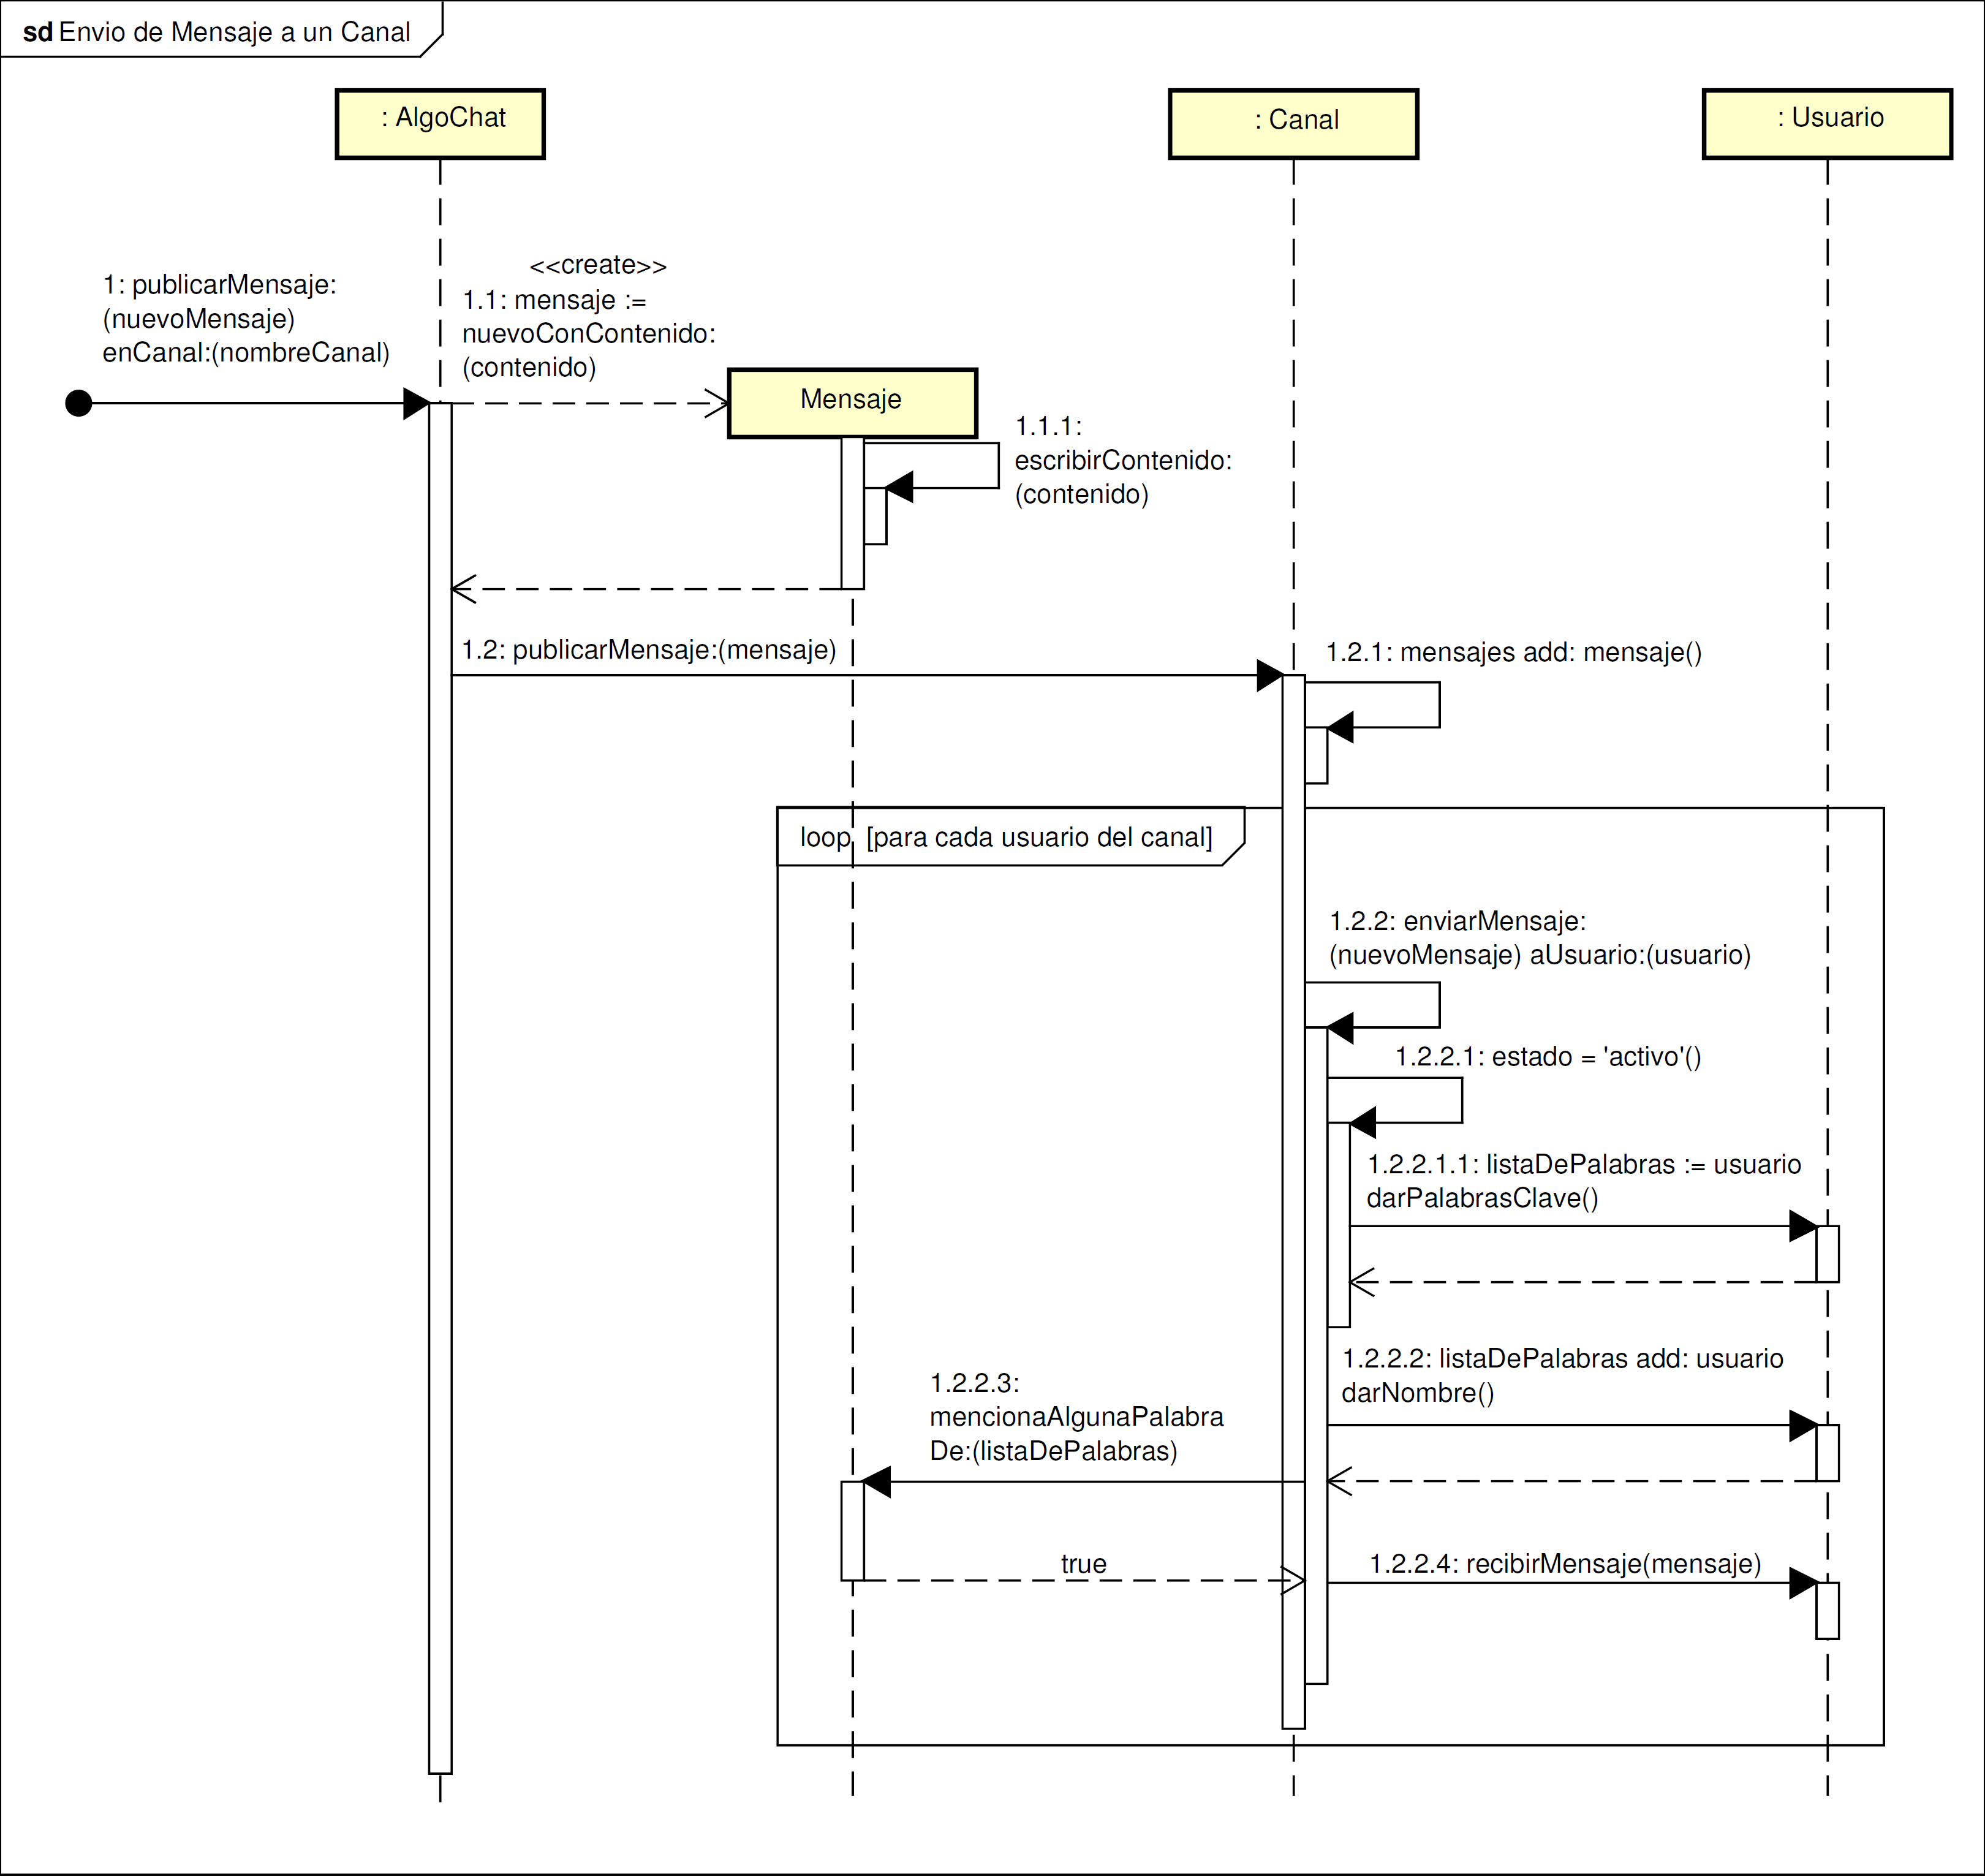
\includegraphics[width=1\textwidth]{diagrama_secuencia01.png}
\caption{\label{fig:seq01}Envió de un \textit{Mensaje} a un \textit{Canal}.}
\end{figure}

En el diagrama de arriba puede observarse como es el proceso para enviar un \textit{Mensaje} nuevo a un \textit{Canal} del chat. El proceso consta de los siguientes pasos:

\begin{enumerate}
	\item Se envía el mensaje \textit{publicarMensaje: nuevoMensaje enCanal: nombreCanal} al \textit{AlgoChat}
	\item El \textit{AlgoChat} crea un nuevo Mensaje con el contenido recibido.
	\item El \textit{AlgoChat} envía el mensaje \textit{publicarMensaje:mensaje} al \textit{Canal} con el \textit{Mensaje} recién creado.
	\item El \textit{Canal} almacena el \textit{Mensaje} recibido en su lista de mensajes, y luego realiza el siguiente \textit{loop} para cada Usuario del \textit{Canal}:
	\begin{enumerate}
		\item Se crea una lista vacía de palabras a buscar en el \textit{Mensaje}.
		\item El \textit{Canal} se envía a si mismo el mensaje \textit{enviarMensaje: nuevoMensaje aUsuario: usuario}. El cual verifica si el \textit{Usuario} se encuentra activo (ver Sección \ref{subsec:implementacionCanal}).
		\begin{itemize}
			\item Caso afirmativo: Solicita al usuario sus palabras clave, enviadole el mensaje \textit{darPalabrasClave}, y las guarda en la lista arriba mencionada. Luego, solicita al usuario su nombre, enviadole el mensaje \textit{darNombre} y lo agrega a la lista anexandole un '@' adelante.
			\item Caso negativo: Unicamente solicita al usuario su nombre.
		\end{itemize}
		\item Envía al \textit{Mensaje} el mensaje \textit{mencionaAlgunaPalabraDe: listaDePalabras} pasandole la lista de palabras a buscar.
		\item Si el \textit{Mensaje} mencionaba alguna de las palabras, se envía el mensaje \textit{recibirMensaje: mensaje} al \textit{Usuario} pasandole el \textit{Mensaje} para que lo guarde.
	\end{enumerate}
\end{enumerate}

\begin{figure}[H]
	\centering
	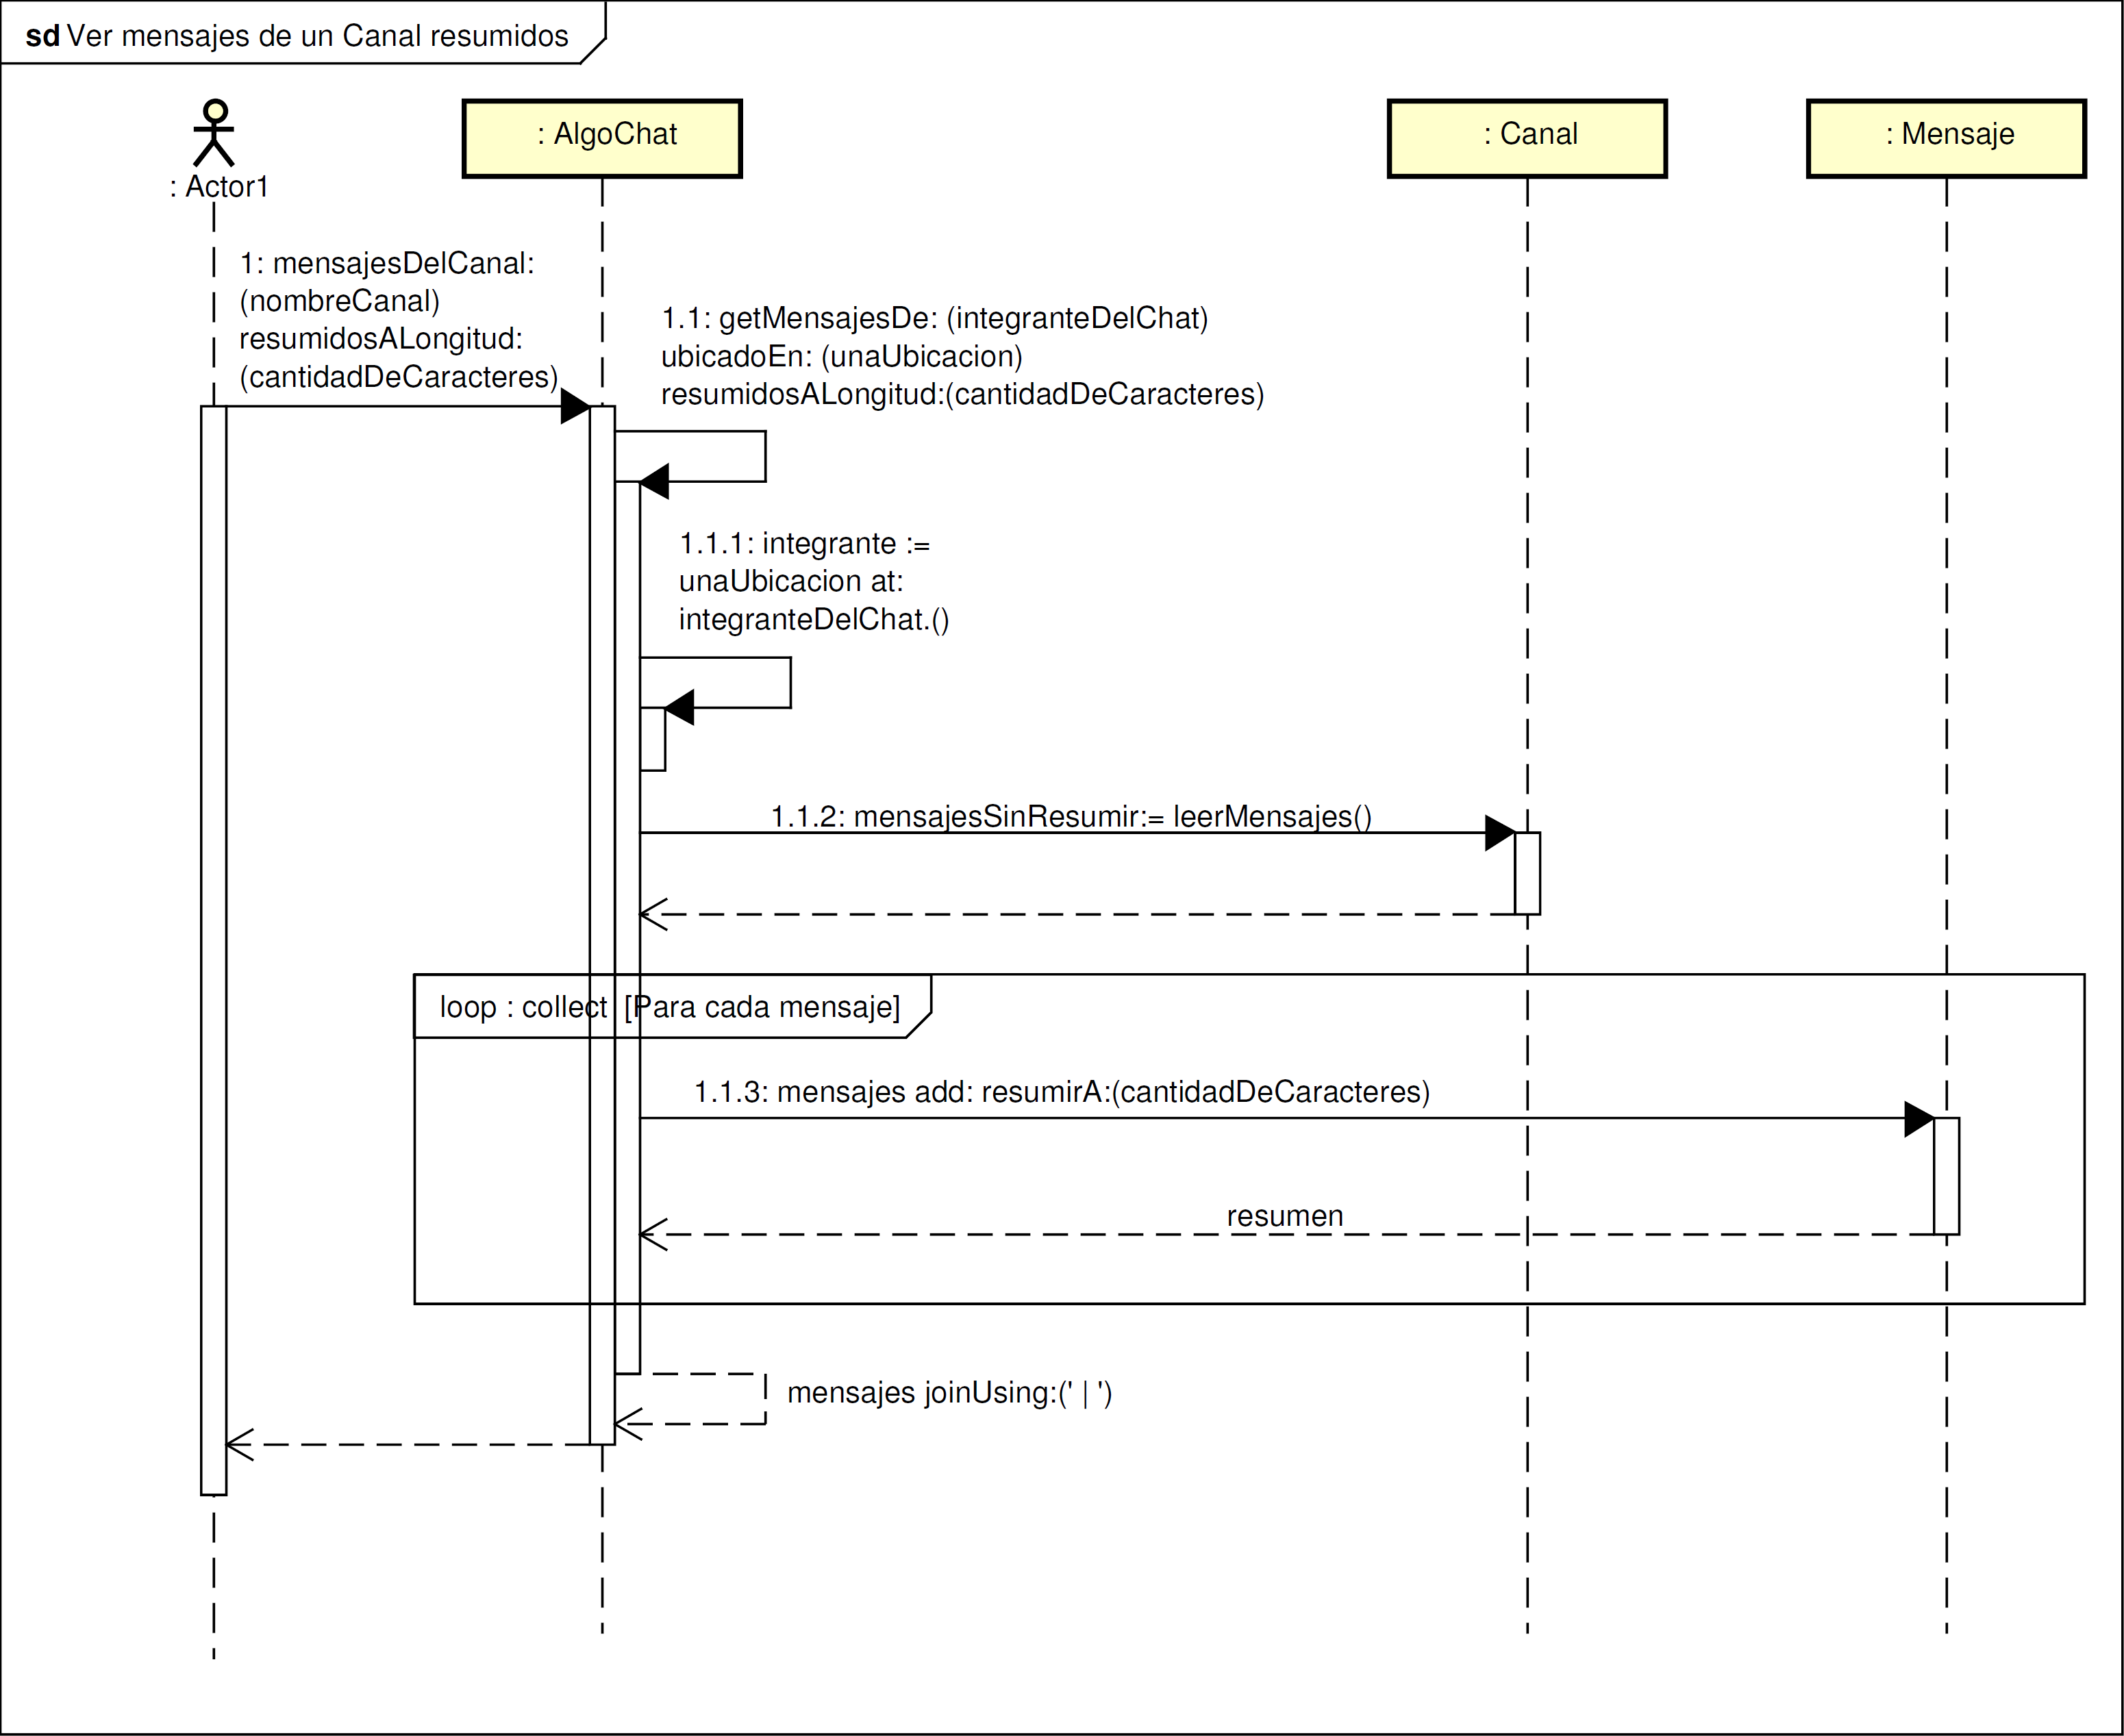
\includegraphics[width=1\textwidth]{diagrama_secuencia02.png}
	\caption{\label{fig:seq02}Ver los \textit{Mensajes} publicados en una \textit{Conversacion}.}
\end{figure}

En el diagrama de arriba puede apreciarse como es el proceso para solicitar a un \textit{Canal} los \textit{Mensajes} publicados en el mismo, resumidos a una cierta cantidad de caracteres cada uno. El proceso es el siguiente:

\begin{enumerate}
	\item Un \textit{Actor} envía al chat el mensaje \textit{mensajesDelCanal: nombreCanal resumidosALongitud: cantidadDeCaracteres}.
	\item El AlgoChat se envia a si mismo el mensaje \textit{getMensajesDe: integranteDelChat ubicadoEn: unaUbicacion resumidosALongitud: cantidadDeCaracteres} el cual puede resumir los\textit{ Mensajes} de cualquier integrante del chat (\textit{Usuario, Conversacion o Canal}) y realiza las siguientes acciones:
	\begin{enumerate}
		\item Guarda en una variable \textit{integrante} al \textit{Canal} del cual se quieren obtener los \textit{Mensajes}.
		\item Envia al \textit{Canal} el mensaje \textit{leerMensajes} que le retorna una lista con todos los \textit{Mensajes} del \textit{Canal}.
		\item Abre un \textit{loop} dentro del cual le envia a cada \textit{Mensaje} del listado recibido el mensaje \textit{resumirA: cantidadDeCaracteres}. Este devuelve el contenido de cada mensaje resumido.
		\item Se almacenan los resúmenes en una nueva lista a medida que avanza el proceso.
	\end{enumerate}
	\item Se devuelve un \textit{String} formado por todos los elementos de la lista de resumidos unidos por pipes. Ej: 'Hola | mundo' 
\end{enumerate}


\section{Excepciones}\label{sec:excepciones}
% Mostrar las secuencias interesantes que hayan implementado. Pueden agregar texto para explicar si algo no queda claro.

No se hizo uso de excepciones en la resolución de este trabajo practico.

\end{document}